\documentclass[tikz,border=6pt]{standalone}
\usepackage{amsmath,amssymb}
\begin{document}
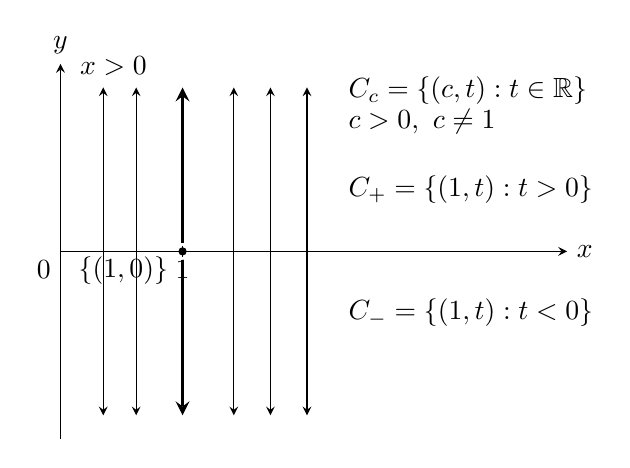
\begin{tikzpicture}[x=1.55cm,y=0.85cm,>=stealth]
  % The group occupies the open half-plane x>0.
  \draw[->] (0,-2.8) -- (0,2.8) node[above] {$y$};
  \draw[->] (0,0) -- (4.15,0) node[right] {$x$};
  \node[anchor=north east] at (0,0) {$0$};
  \node[below] at (1,0) {$1$};
  \draw (1,0.08) -- (1,-0.08);

  % Representative full vertical conjugacy classes for c != 1.
  \foreach \c in {0.35,0.62,1.42,1.72,2.02} {
    \draw[thin,<->] (\c,-2.45) -- (\c,2.45);
  }
  \node[align=left,anchor=west] at (2.28,2.18)
    {$C_c=\{(c,t):t\in\mathbb R\}$\\[-1pt] $c>0,\ c\ne1$};

  % At x=1 the positive and negative rays are different classes.
  \draw[very thick,->] (1,0.13) -- (1,2.45);
  \draw[very thick,->] (1,-0.13) -- (1,-2.45);
  \fill (1,0) circle[radius=1.5pt];
  \node[anchor=west] at (2.28,0.92) {$C_{+}=\{(1,t):t>0\}$};
  \node[anchor=west] at (2.28,-0.92) {$C_{-}=\{(1,t):t<0\}$};
  \node[anchor=east] at (0.96,-0.28) {$\{(1,0)\}$};

  \node[anchor=south west] at (0.08,2.48) {$x>0$};
\end{tikzpicture}
\end{document}
